

\subsection{Aufgabe der Komponente}
Die über SharkNet abgeschickten Nachrichten werden über Bluetooth übertragen. Die Komponente ist dabei ausschließlich für die kabellose Übertragung von Daten bzw. Nachrichten verantwortlich, die Ortung von potentiellen Kommunikationspartern erfolgt über die Wifi-Direct Komponente. Auch die Filterung von bereits bekannten oder semantisch uninteressanten Nachrichten wird nicht innerhalb dieser Komponente, sondern innerhalb der Semantischen Routing Komponente vorgenommen.
\\Da es in SharkNet neben normalen Chats auch Gruppenchats und einen semantischen Broadcast gibt, erfordert der Datenaustausch mit Bluetooth kein Pairing der miteinander kommunizierenden Geräte. Dies trägt maßgeblich zur Benutzerfreundlichkeit bei, da insbesondere beim semantischen Broadcast sonst ständig Anfragen zum Pairing auf dem Gerät erscheinen würden und vom Benutzer zusätzliche Interaktionen erforderlich wären.



\subsection{Architektur}

\subsubsection{Überlick}\label{ch:bluetoothoverview}

Im folgenden UML-Klassendiagramm sind alle Bestandteile der Bluetooth Komponente von SharkNet abgebildet.
\begin{figure}[H]
	\centering
	\hspace*{1cm}
	\makebox[\linewidth][c]{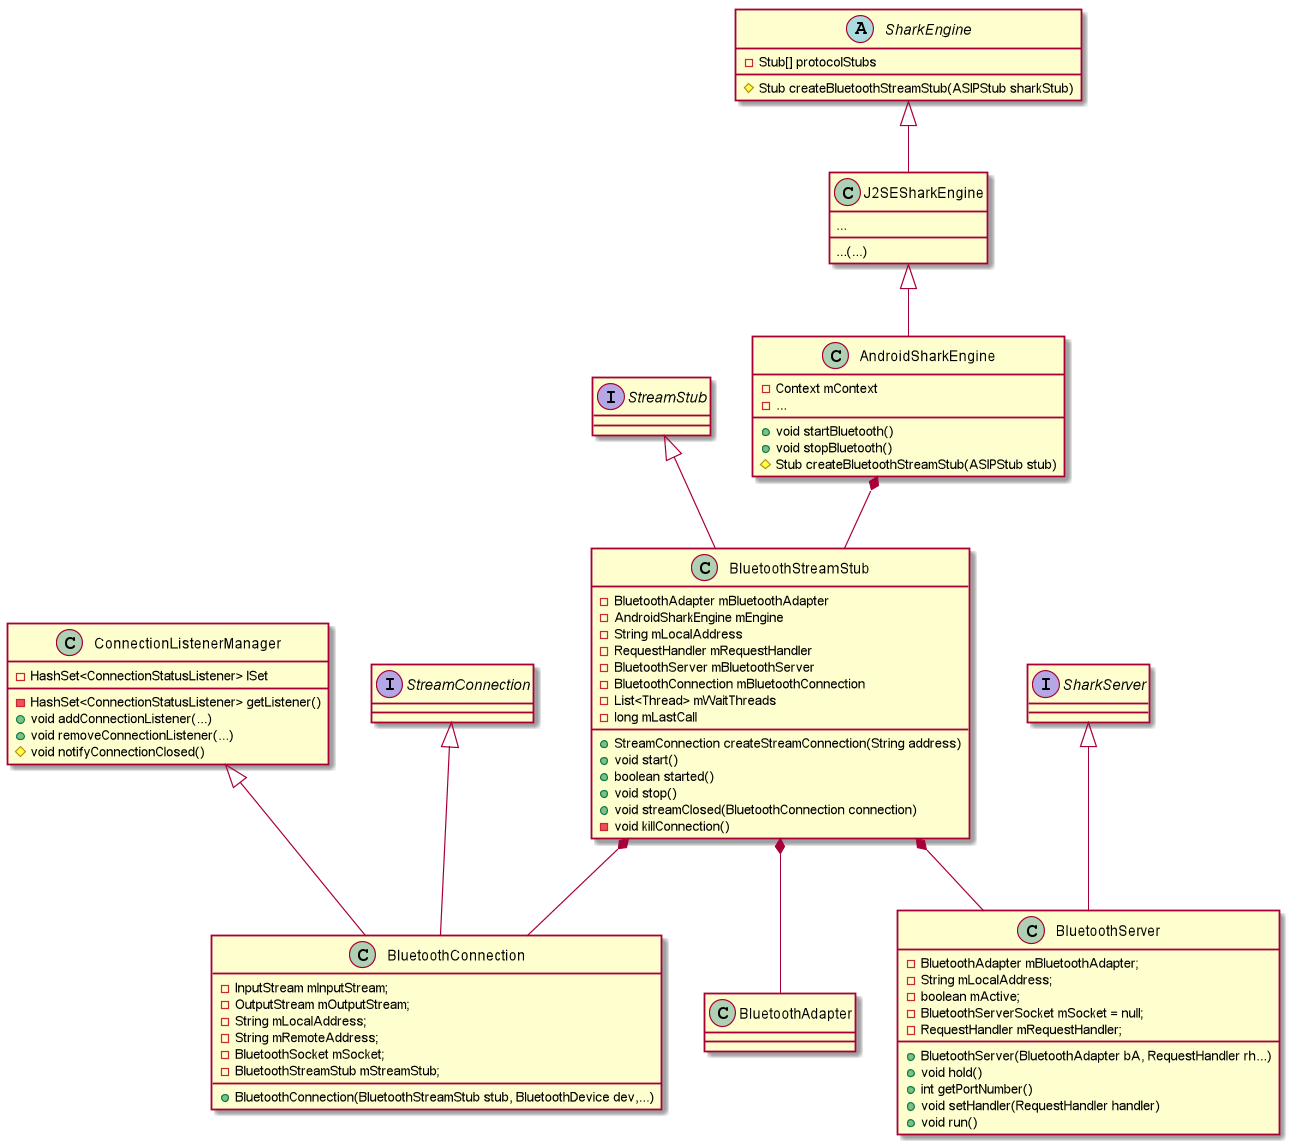
\includegraphics[width=1.1\linewidth]{bluetooth/images/bluetoothGesamt.png}}%
	\caption{Die Bluetooth Klassen im Überblick}
	\label{fig:bluetoothAll}
\end{figure}
Im Zentrum dieser Hierarchie steht die Klasse \textit{BluetoothStreamStub}. Eine Instanz dieser Klasse befindet sich als Attribut in der Klasse \textit{AndroidSharkEngine}, von der aus alle Protokolle wie NFC, Wifi-Direct oder Bluetooth gesteuert werden. Sie stellt daher auch Methoden wie \textit{startBluetooth()} oder \textit{stopBluetooth()} bereit. 





\subsubsection{Schnittstellendefinitionen}\label{ch:bluetoothinterfaces}
Anhand der Klassenhierarchie der Bluetooth-Komponente lässt sich erkennen, dass die folgenden drei Schnittstellen implementiert werden:
\begin{itemize}
	\item \textit{StreamStub}: Mit Hilfe von Implementierungen dieses Interfaces können streambasierte Ende-zu-Ende Verbindungen zwischen zwei Geräten hergestellt werden. Die Klasse BluetoothStreamStub öffnet und schließt daher die Verbindungen zu anderen Geräten per Bluetooth.
	\item \textit{StreamConnection}: Das Shark Framework definiert mit dem Interface StreamConnection das Verhalten einer streambasierten Verbindung zweier Geräte. Dieses Interface ist nicht zu verwechseln mit gleichnamigen Interface von Java ME. Klassen wie \textit{BluetoothConnection}, welche dieses Interface implementieren, bauen in ihren jeweiligen Konstruktur die Verbindung mit ihrem jeweiligen Protokoll auf. In der Klasse \textit{BluetoothConnection} erfolgt dies über das Bluetooth-Protokoll RFCOMM.
	\item \textit{SharkServer}: Eine dieses Interface implementierende Klassen wartet bei der bestehenden Verbindung auf Datenpakete, nimmt diese an und leitet sie an einen \textit{Request Handler} weiter. Die Klasse \textit{BluetoothServer} nimmt daher die Datenpakete an, die per bestehender Bluetoothverbindung eintreffen.

\end{itemize}

\subsection{Nutzung}
Der Start der Komponente erfolgt automatisch mit dem Start der Anwendung durch eine Instanzierung der Klasse \textit{AndroidSharkEngine}. Sie kann jedoch in ebenjener Klasse durch die Methoden \textit{startBluetooth()} und \textit{stopBluetooth()} auch manuell gestartet sowie gestoppt werden.

\subsubsection{Code}
Der Code dieser Komponente kann hier \url{https://github.com/SharedKnowledge/SharkNet-Api-Android/tree/master/api/src/main/java/net/sharksystem/api/shark/protocols/bluetooth} betrachtet werden. Wie auch die anderen Implementierungen von Über\-tra\-gungs\-pro\-to\-kol\-len, befindet sich auch die Bluetooth-Implementierung im Projekt \textit{SharkNet-Api-Android} im Package \textit{protocols}. 
\\Es werden nun die wichtigsten Codezeilen der drei im Unterkapitel Schnittstellendefinitionen erwähnten Klassen beschrieben.
\\Der \textit{BluetoothServer} horcht auf eingehende Verbindungen mit Hilfe der von Android bereitgestellten Klasse \textit{BluetoothSocket}, die folgendermaßen initialisiert wird:
 \lstset{language=Java, caption=Initialisierung des Bluetooth-Server-Sockets, label=DescriptiveLabel, numbers=left, numbersep=1em, breaklines=true, basicstyle=\small}
\begin{lstlisting}
mSocket = mBluetoothAdapter.listenUsingInsecureRfcommWithServiceRecord(BluetoothStreamStub.BT_NAME, BluetoothStreamStub.BT_UUID);
\end{lstlisting}
Hierbei wird mit Hilfe des aktiven \textit{BluetoothAdapter}, welcher auch in der Klasse \textit{BluetoothConnection} benutzt wird, über das Bluetooth-Protokoll \textit{RFCOMM} der Server-Socket erzeugt, zu dem sich andere Geräte verbinden können. Es wird statt der sonst gängigen Methode \textit{listenUsingRfcommWithServiceRecord()} die \textit{insecure} Variante genutzt, um kein Bluetooth-Pairing zwischen den Geräten vorher durchführen zu müssen. Der nächste Auszug zeigt die Annahme von eingehenden Verbindungen auf Serverseite:
 \lstset{language=Java, caption=Serverseitige Annahme der Bluetooth-Verbindungen (Auszug), label=DescriptiveLabel, numbers=left, numbersep=1em, breaklines=true, basicstyle=\small}
\begin{lstlisting}
try {
  while (mActive){
    BluetoothSocket bluetoothSocket = mSocket.accept();
    BluetoothConnection con = new BluetoothConnection(bluetoothSocket, mLocalAddress);
    mRequestHandler.handleStream(con);
  }
  mSocket.close();
\end{lstlisting}
Die Annahme der Anfrage geschieht in der dritten Zeile, wobei der daraus resultierende \textit{BluetoothSocket} in der folgenden Zeile für den Aufbau einer Verbindung genutzt wird. Die Verbindung wird anschließend vom Shark-Interface \textit{RequestHandler} verwertet. Dies bedeutet, dass die im Stream enthaltene Nachricht innerhalb der Framework-Ebene nun weiterverarbeitet wird. Dies schließt unter anderem auch die semantische Auswertung der Nachricht mit ein.
\\Der Aufbau einer Bluetooth-Verbindung erfolgt auf Clientseite ähnlich zum Aufbau auf der Serverseite innerhalb der Klasse \textit{BluetoothConnection}:
 \lstset{language=Java, caption=Clientseitige Initialisierung des Sockets, label=DescriptiveLabel, numbers=left, numbersep=1em, breaklines=true, basicstyle=\small}
\begin{lstlisting}
mSocket = device.createInsecureRfcommSocketToServiceRecord(BluetoothStreamStub.BT_UUID)
\end{lstlisting}
Auch hier wird die \textit{Insecure} Variante der Methode genommen, um auf ein Pairing verzichten zu können.
\\Instanzen der beiden bisher vorgestellten Klassen \textit{BluetoothServer} und \textit{BluetoothStreamStub} werden durch die Klasse \textit{BluetoothStreamStub} erzeugt und verwaltet. Neben der Erzeugung dieser Objekte liefert der \textit{BluetoothStreamStub} weiterhin die lokale Bluetooth MAC-Adresse des Geräts:
\textit{BluetoothConnection}:
\lstset{language=Java, caption=Auslesen der Bluetooth MAC-Adresse, label=DescriptiveLabel, numbers=left, numbersep=1em, breaklines=true, basicstyle=\small}
\begin{lstlisting}
mLocalAddress = android.provider.Settings.Secure.getString(engine.getContext().getContentResolver(), "bluetooth_address");
//mLocalAddress = BluetoothAdapter.getDefaultAdapter().getAddress() Nur vor Marshmallow nutzbar, liefert nach dieser Version nur eine unbrauchbare Konstante!
\end{lstlisting}
Dies geschieht zwangsweise über eine Reflektion, da die bis Android-Marshmallow dafür vorhergesehene Methode nur eine Konstante liefert, die nicht der eigentlichen Bluetooth MAC-Adresse des Geräts entspricht. Die Bluetooth MAC-Adresse wird jedoch zwingend für \textit{Insecure} Verbindungen benötigt, welche kein Bluetooth-Pairing erfordern, was für die Broadcast-Komponente essentiell ist. 
\\Die restlichen Methoden der Bluetooth-Komponente wie beispielsweise \textit{killConnection()} sind mnemonischer Natur.

\subsubsection{Deployment / Runtime}
[...]


\subsection{Test}
\subsubsection{Gerätetest}
Mit den folgenden Android-Geräten ist die Komponente auf Kompatibilität geprüft worden:
\begin{table}[H]
	\begin{center}
		\caption{Kompatibilitätstest der Komponente}
		\label{tab:dimensions}
		\begin{tabular}{l|c|c} 			
			Gerät & Android-Version & kompatibel \\
			\hline
			LG Nexus 5x & 8.0 & Ja\\
			LG Nexus 5x & 8.1 & Nein\\
			LG Nexus 5 & 6.1 & Ja\\
			Sony Xperia XZ Premium & 8.0 & Ja\\
			Sony Xperia Z4 Tablet & 7.1.1 & Ja\\
			Lenovo B & 6.0 & Ja\\
			Lenovo A5500-F Tablet & 4.4 & Nein\\
			Raspberry Pi 3 & 6.0.1 & Ja\\	
			Wandboard Quad & 5.0.2 & Ja\\			
		\end{tabular}
	\end{center}
\end{table}
Seit neusten Android-Version 8.1 ist es nicht mehr mit der in Listing 4.4 beschriebenen Refeklektion möglich, die Bluetooth MAC-Adresse programmatisch auszulesen. Dementsprechend kann das Testgerät Nexus 5x seit dem Update des Betriebssystems keine Nachrichten via Bluetooth mehr empfangen, da die anderen Geräte keine valide MAC-Adresse vom Nexus 5x erhalten haben und die Verbindung somit ohne Pairing nicht erfolgreich aufgebaut werden kann. 
\\Beim Lenovo A5500-F Tablet handelt es sich um eine zu alte Android-Version, wodurch in mehreren Komponenten zu Exceptions kommt, weil benötigte Methoden noch nicht enthalten sind.



\subsection{Ausblick}
Es ist empfehlenswert, die von Android gestellten Bluetooth Klassen durch die dazu äquivalenten Bluetooth Low Energy (BLE) Klassen entweder zu ersetzen oder zumindest eine Alternative zu dem klassischen Bluetooth Package zu bieten. BLE verbraucht weit weniger Akkuleistung als das klassische Bluetooth, kann dafür aber nur eine geringere Menge an Daten pro Verbindung unterstützen. Da die mit SharkNet verschickten Nachrichten auch trotz der semantischen Annotationen nur wenige Kilobyte benötigen, stellt dies für SharkNet kein Hindernis dar.
\\Notwendig ist zukünftig außerdem das Ersetzen der in Listing 4.4 dargestellten Reflektion zum Auslesen der Bluetooth MAC-Adresse. Dies funktioniert nur mit Geräten bis einschließlich Android 8.0, ab Android 8.1 ist die ausgelesene MAC-Adresse inkorrekt. Über die WiFi-Komponente an andere Geräte versendete inkorrekte Bluetooth-Adressen führen dann dazu, dass das Gerät keine Nachrichten über Bluetooth empfangen kann. 
\\Lasttests mit mehreren miteinander kommunizierenden Geräten und gleichzeitigem Spammen von Nachrichten haben der Komponente ebenfalls Grenzen der Belastbarkeit aufgezeigt. So können bei zu hoher Last Nachrichten verloren gehen, da das Empfangsgerät die in Listing 4.2 gezeigte \textit{accept()} Methode nicht aufgerufen wird. 
\newpage

